It looks like there is a tipping point at the frequency of $10^{7.5}$ or 7.5 in log space. From here I got a different scaling for each of the two sections of the distribution.

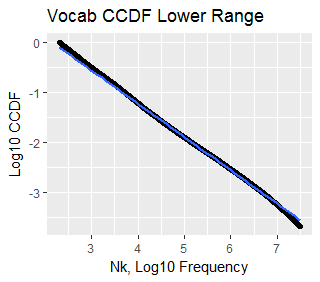
\includegraphics{Problem2_lower_range.png}

Linear regression from the upper interval reveals a $\gamma$ value with a 95\% confidence interval of
$$
    1.499889 < \gamma < 1.499471
$$
resulting in,

$$
    0.499889 < \gamma - 1 < 0.499471
$$

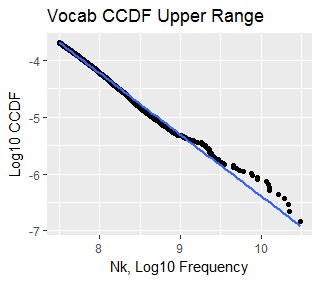
\includegraphics{Problem2_upper_range.png}

From the upper range of the distribution, linear regression with a 95\% confidence interval gives a $\gamma$ value of,
$$
    0.9320839 < \gamma < 0.9265242
$$
resulting in,
$$
    -0.0679161 < \gamma - 1 < -0.0734758
$$